\documentclass{book}  % fundamental class file is 'book'.
\usepackage{piers}  % use the file 'piers.sty'.
\pagestyle{piers}


\usepackage{hyperref}
\usepackage{cite}
\usepackage{amsmath}
%\interdisplaylinepenalty=2500 % suggested by IEEE to use with amsmath package
\usepackage{amsfonts}
\usepackage{graphicx}
\usepackage{subfigure}
\usepackage{epstopdf}

\usepackage[T1]{fontenc} % optional
\usepackage[cmintegrals]{newtxmath}
\usepackage{bm} % optional


% ================ self-defined command ==================
\usepackage{color} % for marking text
\newcommand{\highlight}[1]{\Huge\textcolor{red}{#1}\normalsize}
\newcommand{\defaultfigurewidth}{0.5\columnwidth}
% --------- fix non-conventional piers command -----------
% So you can simply use abstract, section, and subsection
% as used in IEEE papers.
\newenvironment{abstract}{\begin{piersabstract}}{%
	\end{piersabstract}\ignorespacesafterend% as suggested above
}
\renewcommand{\section}[1]{\psection{#1}}
\renewcommand{\subsection}[1]{\psubsection{#1}}


% correct bad hyphenation here
\hyphenation{op-tical net-works semi-conduc-tor}

\begin{document}

\title{Design of High Speed Link System}
\maketitle

%=== List of authors (in order) ========
%-- Author(s) for the first affiliation ---
\author      {Chang-Pao Chang}
\affiliation {University of Illinois at Urbana-Champaign}
\address     {}% optional
\city        {Boston}
\postalcode  {}% optional
\country     {USA}
\phone       {345566}    % optional
\fax         {233445}    % optional
\email       {cchang95@uiuc.edu}  % optional
\misc        { }  % optional
\nomakeauthor
%------------------------------------

%=== List of authors (in order) ========
%-- Author(s) for the second affiliation ---
\author      {Xiou Ge}
\affiliation {University of Illinois at Urbana-Champaign}
\address     {}% optional
\city        {Urbana}
\postalcode  {61801} % optional
\country     {USA}
\phone       {} % optional
\fax         {} % optional
\email       {xiouge2@uiuc.com}  % optional
\misc        { }  % optional
\nomakeauthor
%-------------------------------------

%---Output of Authors----------------------
\begin{authors}	
	{\bf Chang-Pao Chang}$^{1}$, {\bf Xiou Ge}$^{2}$\\
	\medskip
	$^{1}$cchang95@uiuc.com\\
	$^{2}$xiouge2@uiuc.com	
\end{authors}
%--------------------------


%---Content of Paper Abstract-----------------------
\begin{paper}
	
\begin{abstract}
	
\end{abstract}
%
\section{Introduction}
\label{sec:Intro}

\section{System Level Design}
\label{sec:system}

\section{Channel Design}
\label{sec:channel_design}

Since the target bit rate is quite high (3Gbps), we used one of the low loss substrate to design our PCB. The RO4003 from Rogers company is widely used to design various high frequency circuit \cite{na_ro4003_rogers}. We use PCB of 9 layers of metal. Fig.~\ref{fig:pcb_layers} shows the dimensions of each layers. The top and bottom layer are the signal layer, and the rest 7 layers at the middle of the PCB are simulated as ground layer. These ground layers were later connected using grounded vias. Each layer is of 19 mil height, and the thickness of metal is 1 mil. \\

As for package, we use one layer of thin-film ceramic from Murawa \cite{na_alumina_substratess}. The substrate is far more thinner than those used in PCB. Table.~\ref{table:material} shows the material properties used for PCB and package.

\begin{table}[h]
	\renewcommand{\arraystretch}{1.3}
	\caption{Material properties used for channel design.}
	\vskip0.2in
	\begin{center}
		\begin{tabular}{| l | l | l | l | c | c | c | c | c |}
			\hline
			Usage   & Substrate  & Trace & Metal Layers & $\varepsilon_r$ & $\tan\delta$ & $r\_via$ & $h\_pcb$ & $t\_pcb$\\ \hline
			PCB     & RO4003  \cite{na_ro4003_rogers} & Copper & 9 & 3.8 & 0.02 & 20 mil & 19 mil & 1 mil \\ \hline
			Package & Alumina \cite{na_alumina_substratess} & Copper & 2 & 9.8 & 0.02 & 150um & 200 um & 17 um \\
			\hline
		\end{tabular}
	\end{center}
	\label{table:material}			
\end{table}


\subsection{PCB Traces}
\label{subsec:pcb_traces}
The differential PCB traces are designed such that the single line impedance is 50 $\Omega$, and the differential impedance is 100 $\Omega$. Fig.~\ref{fig:pcb_trace} shows the design parameters to achieve the desired impedance. The 2D extraction tool, Ansys Q2D is used to analyze and fine-tune the parameters. Fig.~\ref{fig:pcb_trace_impedance} shows the impedance of the differential line up to 40GHz. It shows that the differential impedance is 96$\Omega$ while the common impedance is 25$\Omega$ at 10GHz. 


\begin{figure}[htbp!]
	\centering
	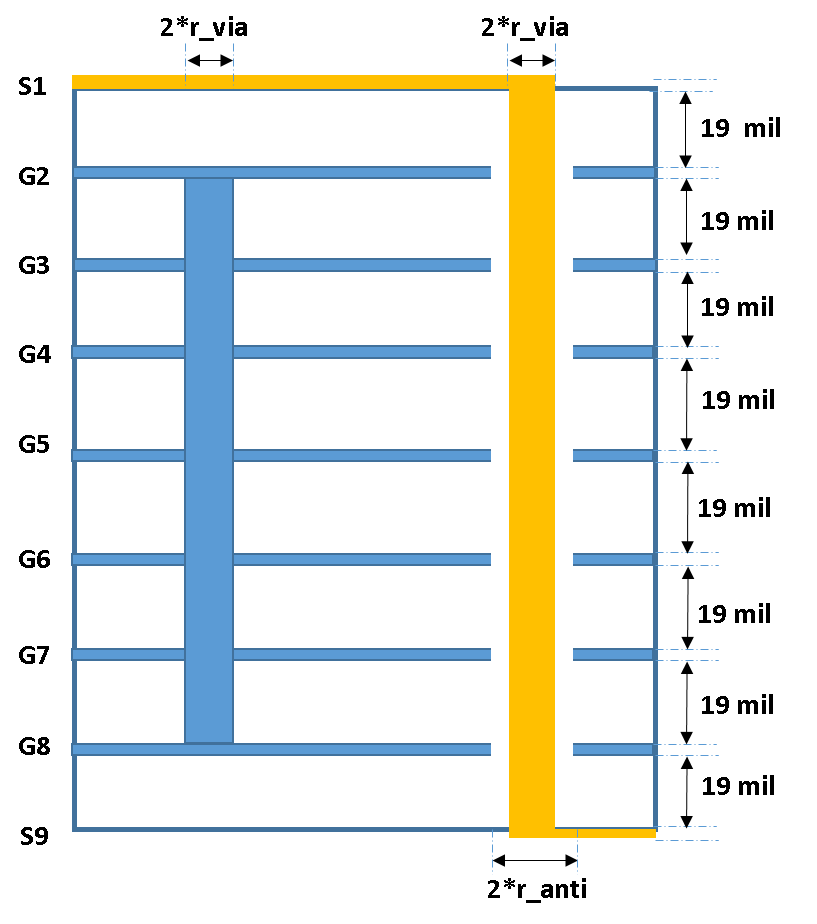
\includegraphics[width=0.8\columnwidth]{./img/PCB/PCB_layer_dimension.png}
	\caption{Dimension and layers in designated PCB. $r\_via=20 mil$ is the radius of both signal and ground via. The height of each PCB layer is 19 mil, and the thickness of copper is 1 mil. }
	\label{fig:pcb_layers} % label must put at the last
\end{figure}

\begin{figure}[htbp!]
	\centering
	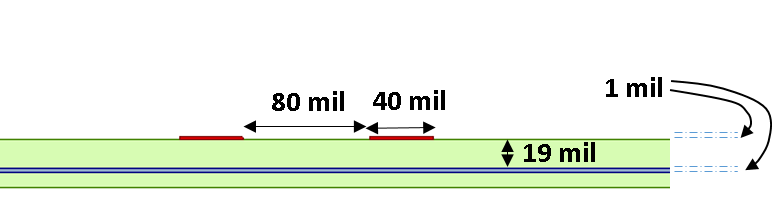
\includegraphics[width=0.8\columnwidth]{./img/PCB/differential_PCB_2D_CrossSection.png}
	\caption{Design parameter of PCB traces.}
	\label{fig:pcb_trace} % label must put at the last
\end{figure}

\begin{figure}[htbp!]
	\centering
	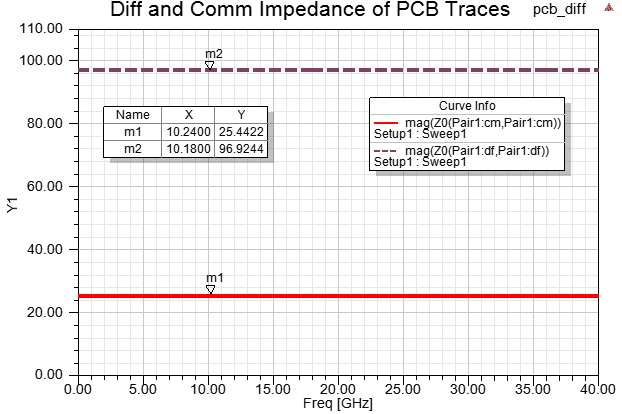
\includegraphics[width=0.8\columnwidth]{./img/PCB/differential_PCB_2D_impedance.png}
	\caption{Differential and common impedance of designated PCB traces. Solid: common mode impedance; dash: differential mode impedance.}
	\label{fig:pcb_trace_impedance} % label must put at the last
\end{figure}


\subsection{Via Transition}
Since there will be a via transition from top to the bottom of the PCB, the strong discontinuity of this via transition will cause strong reflection, as shown in Fig.~\ref{fig:pcb_layers}. The entire structure, however, can be modeled using quasi-static approach. The via itself can be modeled as lumped resistance and inductance, and the parasitic capacitance distributed around the via to the ground plane surrounded. Fig.~\ref{fig:pcb_via_tran_LC} shows the quasi-static models of via transition. Fig.~\ref{fig:pcb_via_lump} shows the lumped model of via transition of differential line. \\

The 3D quasi-static extraction tool Ansys Q3D \cite{na_ansys_q3d} is used to extract the lumped element of these conductor. Fig.~\ref{fig:pcb_via_tran_Q3D} shows the via transition model for Q3D extraction. Since the structure is symmetry, to lower the reflection, a simple approximation can be used. The lumped differential impedance defined in \ref{eq:pcb_via_tran_lump_diff} is set to be 100 $\Omega$. This can be achieved through adjusting the radius of anti-pad, $r\_anti$ in Fig.~\ref{fig:pcb_layers}.

\begin{equation}\label{eq:pcb_via_tran_lump_diff}
Z^{lump}_{diff}\equiv \sqrt{\frac{L_{11} - L_{12}}{C_{11} + \left|C_{12}\right|}} = 100\Omega
\end{equation}

\begin{figure*}[h]
	\centering	
	\subfigure[Via transition in Q3D]{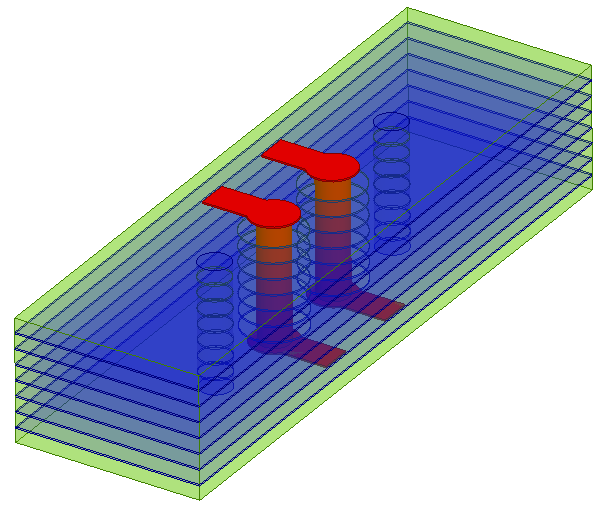
\includegraphics[width=0.5\textwidth]{./img/PCB/Via_Transition/Q3D_tuned_side.png}}%
	\subfigure[Via transition in Q3D]{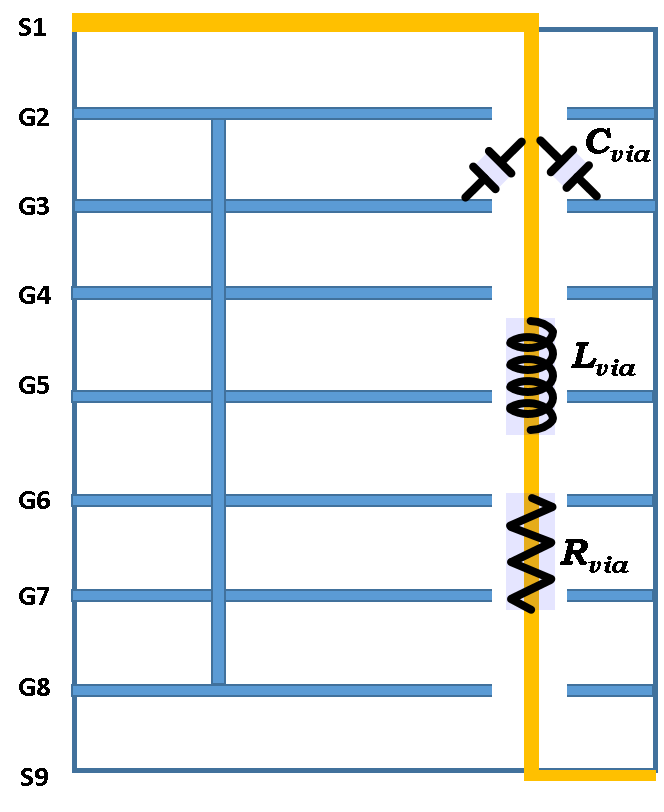
\includegraphics[width=0.5\textwidth]{./img/PCB/Via_Transition/Via_transition_LC_modeling.png}}
	\subfigure[Lumped Model]{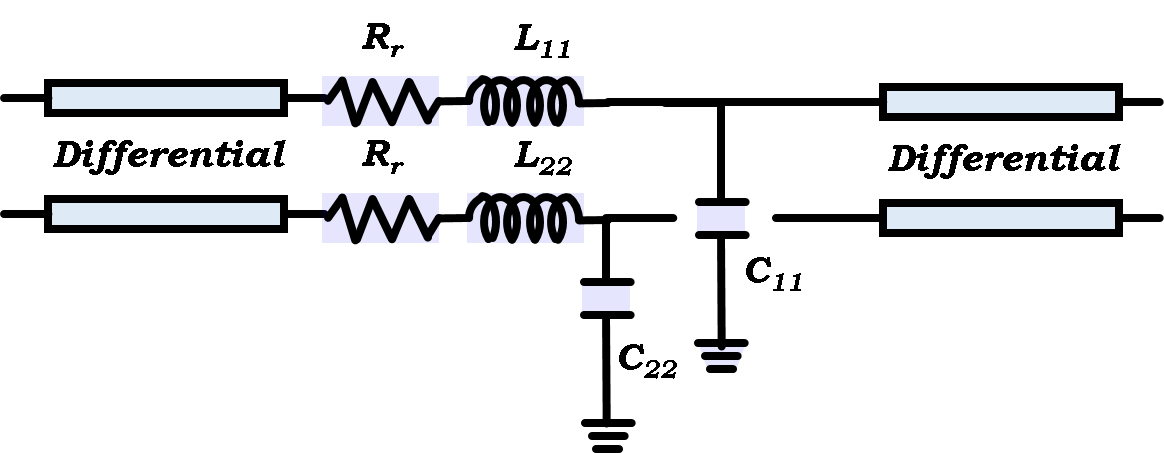
\includegraphics[width=\textwidth]{./img/PCB/Via_Transition/lumped_model.png}}%
	\caption{Via transition model for Q3D extraction}
\end{figure*}

\highlight{Add Q3D preliminary result}

The preliminary result given in Q3D is later imported into HFSS for full-wave simulation. Fig.~\ref{fig:pcb_via_trans_HFSS} shows the structure used in HFSS, and Fig.~\ref{fig:pcb_via_tran_S} shows the S parameter of differential and common mode. The high level of $S^{cc}_{11}$ shows good common mode rejection, around -10dB, below 10GHz, while the $S^{dd}_{11}$ remains below -20dB below 10GHz. Fig.~\ref{fig:pcb_via_tran_Sdd11_smith} shows the smith chart of $S^{dd}_{11}$. The low reflection of differential mode can be observed that the reflection is below 0.26 with 10GHz.

\begin{figure*}[h]
	\centering
	\subfigure[Tilted view]{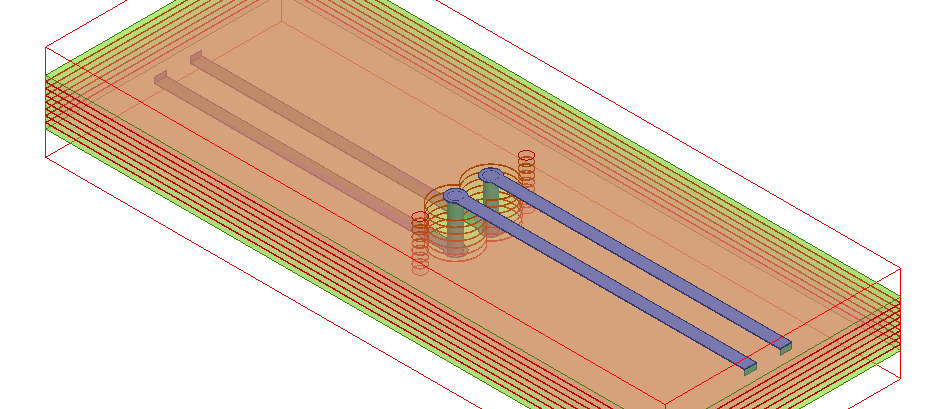
\includegraphics[width=0.5\textwidth]{./img/PCB/Via_Transition/View_45_Degree.png}}%
	\subfigure[Top view]{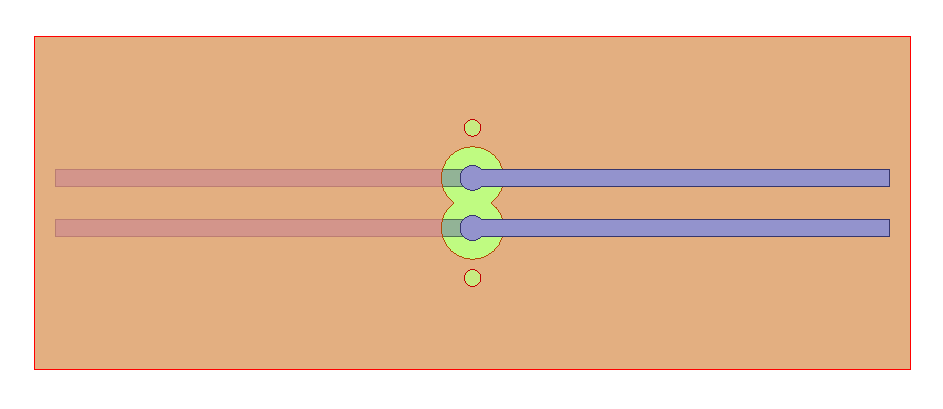
\includegraphics[width=0.5\textwidth]{./img/PCB/Via_Transition/View_Top.png}}%
	\label{fig:pcb_via_trans_HFSS}
	\caption{Via transition simulated in HFSS.}
\end{figure*}


\begin{figure}[h]
	\centering
	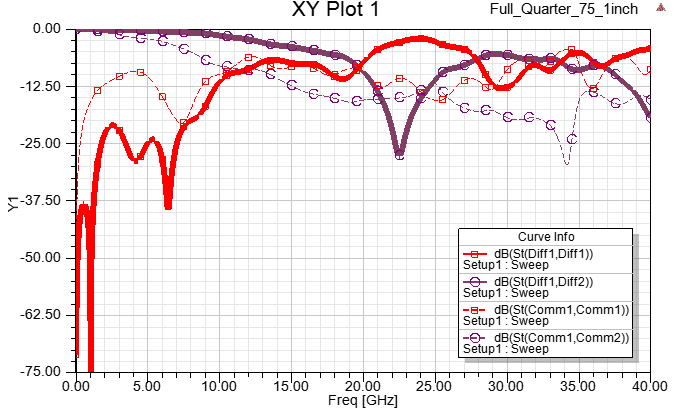
\includegraphics[width=0.8\columnwidth]{./img/PCB/Via_Transition/S_parameter.png}
	\caption{S parameter of via transition in PCB. $r\_anti = 75 mil$. }
	\label{fig:pcb_via_tran_S} % label must put at the last
\end{figure}

\begin{figure}[htbp!]
	\centering
	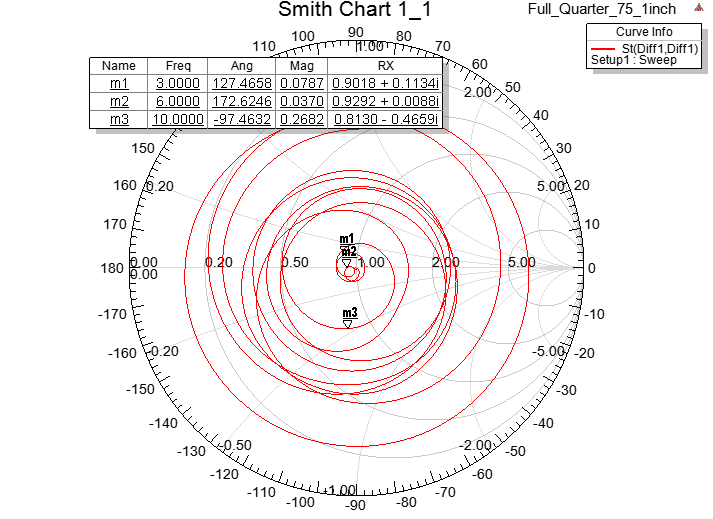
\includegraphics[width=0.8\columnwidth]{./img/PCB/Via_Transition/via_transition_smith.png}
	\caption{Smith chart of $S^{dd}_{11}$ of via transition in PCB. $r\_anti = 75 mil$. }
	\label{fig:pcb_via_tran_Sdd11_smith} % label must put at the last
\end{figure}

\subsection{Package Traces}
Similar procedure described in \ref{subsec:pcb_traces} can also be applied to the designation of traces on packages. The material properties of substrate used in package is described in Table.~\ref{table:material}.  Fig.~\ref{fig:pkg_trace} shows the design parameters to achieve the desired impedance, and Fig.~\ref{fig:pkg_trace_impedance} shows the impedance of the differential line up to 40GHz. It shows that the differential impedance is 96$\Omega$ while the common impedance is 25$\Omega$ at 10GHz.

\begin{figure}[htbp!]
	\centering
	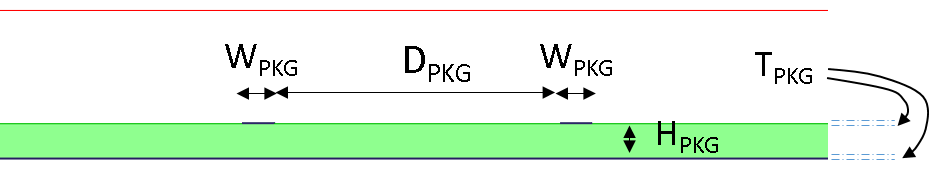
\includegraphics[width=0.8\columnwidth]{./img/PCB/differential_PKG_2D_CrossSection.png}
	\caption{Design parameter of package traces.}
	\label{fig:pkg_trace} % label must put at the last
\end{figure}

\begin{figure}[htbp!]
	\centering
	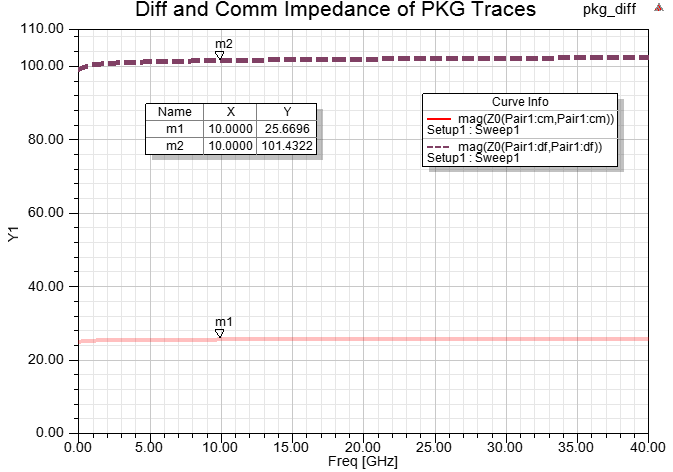
\includegraphics[width=0.8\columnwidth]{./img/PCB/differential_PKG_2D_impedance.png}
	\caption{Differential and common impedance of designated PCB traces. Solid: common mode impedance; dash: differential mode impedance.}
	\label{fig:pkg_trace_impedance} % label must put at the last
\end{figure}

\subsection{Bonding Wire Transition}
\label{sec:bond_wire}
The transition between package and PCB is through using bonding wire. The radius of bonding wire is 25um. 




\section{Feed Forward Equalizer}
\label{sec:FFE}

\section{Decision Feedback Equalizer}
\label{sec:DFE}

\section{Differential Amplifier}
\label{sec:diff_Op}

\section{Result}
\label{sec:result}



\section{Conclusion}
In this paper, we use the vector electric field formulation, combined with both edge and element basis, to analyze several type of waveguide structure. Both homogeneous and inhomogeneous  waveguide shows a good agreement to the analytic solution. In addition, the slow wave factors of MIS structure are analyzed with different substrate loss. The transitions from slow wave mode to quasi-TEM mode or skip-depth mode can be clearly observed. 

% =============  Reference Section ==============

\bibliographystyle{IEEEtran}
\bibliography{IEEEabrv,F:/SoftwarePC/AutoupdateZoteroLibrary}

%\begin{thebibliography}{99}	
%
%\end{thebibliography}

\end{paper}
\end{document}

